\documentclass[rgb,dvipsnames]{beamer}
\usepackage[english]{babel}
\usepackage[utf8]{inputenc}
\usepackage{xcolor}
\usepackage{listings}
\usepackage{adjustbox}
\usepackage{amsmath}
\usepackage{multirow}
\usepackage{tikz}
\usepackage[linewidth=1pt]{mdframed}

% Graphics
\usepackage{graphicx}

\usepackage{fancyvrb}

% Font
\usepackage{paratype}
\setbeamerfont{frametitle}{family=\bf}

% Beamer theme settings
\usecolortheme{seagull}
\usenavigationsymbolstemplate{} % no navigation buttons

\newcommand{\Fn}{\ensuremath{\lambda}}

\lstdefinelanguage{Futhark}
{keywords={fun,if,then,else,loop,do,map,reduce,filter,scan,redomap,transpose,rearrange,reshape,iota,replicate,let,in,for,while,with,f32,i32,i8,u8,zip,stream_red,unsafe,local},%
  sensitive=true,%
  comment=[l]{--},%
  string=[b]",%
  literate={\\}{\Fn}{1} {->}{$\rightarrow$}{1} {<-}{$\leftarrow$}{1},
  moredelim=**[is][\color{red}]{@}{@},
  moredelim=**[is][\color{blue}]{!}{!},
}

\lstdefinelanguage{none}{
  identifierstyle=
}

\lstset{
  language=Futhark,
  basicstyle=\footnotesize
}

% code highlighting commands in own block
\DefineVerbatimEnvironment{code}{Verbatim}{fontsize=\scriptsize}
\DefineVerbatimEnvironment{icode}{Verbatim}{fontsize=\scriptsize}

% Fancy code with color commands:
\DefineVerbatimEnvironment{colorcode}%
        {Verbatim}{fontsize=\scriptsize,commandchars=\\\{\}}

%%%%%%%%%%%%%%%%%%%%%%%%%%%%%%%%%%
%%%%%    some coloring    %%%%%%%%

\definecolor{Red}{RGB}{220,50,10}
\definecolor{Blue}{RGB}{0,51,102}
\definecolor{Yellow}{RGB}{102,51,0}
\definecolor{Orange}{RGB}{178,36,36}
\definecolor{Grey}{RGB}{180,180,180}
\definecolor{Green}{RGB}{20,120,20}
\definecolor{Purple}{RGB}{160,50,100}
\newcommand{\red}[1]{\textcolor{Red}{{#1}}}
\newcommand{\blue}[1]{\textcolor{Blue}{{#1}}}
\newcommand{\yellow}[1]{\textcolor{Yellow}{{#1}}}
\newcommand{\orange}[1]{\textcolor{Orange}{{#1}}}
\newcommand{\grey}[1]{\textcolor{Grey}{{#1}}}
\newcommand{\green}[1]{\textcolor{Green}{{#1}}}
\newcommand{\purple}[1]{\textcolor{Purple}{{#1}}}




% use "DIKU green" from our color theme for \emph
\renewcommand{\emph}[1]{\textcolor{structure}{#1}}
% use some not-too-bright red for an \emp command
\definecolor{DikuRed}{RGB}{130,50,32}
\newcommand{\emp}[1]{\textcolor{DikuRed}{ #1}}
\definecolor{CosGreen}{RGB}{10,100,70}
\newcommand{\emphh}[1]{\textcolor{CosGreen}{ #1}}
\definecolor{CosBlue}{RGB}{55,111,122}
\newcommand{\emphb}[1]{\textcolor{CosBlue}{ #1}}
\definecolor{CosRed}{RGB}{253,1,1}
\newcommand{\empr}[1]{\textcolor{CosRed}{ #1}}

\newcommand{\mymath}[1]{$ #1 $}
\newcommand{\myindx}[1]{_{#1}}
\newcommand{\myindu}[1]{^{#1}}


\title{Introduction to Data-Dependency Analysis}
%\subtitle{Purely Functional GPU-Programming with Nested Parallelism and In-Place Array Updates}
\date{28th of November 2017}
\author{Cosmin E. Oancea\\cosmin.oancea@diku.dk}
\institute{}

\begin{document}

\usebackgroundtemplate{
\tikz[overlay,remember picture] \node[opacity=0.4, at=(current page.center)] {
   
\includegraphics[height=\paperheight,width=\paperwidth]{figures/neuro-image.jpg}};
    %{images/JellingStoneTextside.jpg}};
}

\frame{\titlepage}

\usebackgroundtemplate{}

\begin{frame}
  \frametitle{Material}

``Parallel Computer Organization and Design'', Michel Dubois, Murali Annavaram, and Per Stenstr\"om, 
%ISBN 978-521-88675-8. 
Cambridge University Press, 2012.
\bigskip
\bigskip

``Optimizing Compilers for Modern Architectures'', Randy Allen and Ken Kennedy, Morgan Kaufmann, 2001.

\end{frame}

\begin{frame}
  \frametitle{Dependency Analysis: Motivation}

  \begin{itemize}
    \item Moore's Law still in effect via parallelism scaling.\bigskip
    \item All modern architectures adopt some form of parallelism,\\
            but are getting more and more capricious.\bigskip

\begin{center}
\unitlength0.3em
\begin{picture}(100,20)
\put(0,0){\framebox(15,4){Fortran}}
\put(0,8){\framebox(15,4){Pencil}}
\put(0,16){\framebox(15,4){Obsidian}}

\put(15,2){\vector(2,1){15}}
\put(15,10){\vector(1,0){15}}
\put(15,18){\vector(2,-1){15}}

\put(30,8){\framebox(22,4){Compilers}}
%\put(30,6){\framebox(22,8){\parbox[b][4em][c]{0.15\textwidth}{Dependency \\ Analyses} }}

\put(52,10){\vector(2,1){15}}
\put(52,10){\vector(1,0){15}}
\put(52,10){\vector(2,-1){15}}

\put(67,0){\framebox(15,4){FPGA}}
\put(67,8){\framebox(15,4){Many-Core}}
\put(67,16){\framebox(15,4){Multi-Core}}

%\uncover<2->{
%\qbezier(45,8)(55,0)(40,0)
%\qbezier(40,0)(25,0)(35,8)
%\put(35,8){\vector(1,1){0}}
%}
\end{picture}
\end{center}
    \bigskip
    \item What is the basis for deriving a correct and efficient translation?

  \end{itemize}

  

\end{frame}

\begin{frame}
  \frametitle{Dependency Analysis: Motivation}

  \begin{itemize}
    \item Moore's Law still in effect via parallelism scaling.\bigskip
    \item All modern architectures adopt some form of parallelism,\\
            but are getting more and more capricious.\bigskip

\begin{center}
\unitlength0.3em
\begin{picture}(100,20)
\put(0,0){\framebox(15,4){Fortran}}
\put(0,8){\framebox(15,4){Pencil}}
\put(0,16){\framebox(15,4){Obsidian}}

\put(15,2){\vector(2,1){15}}
\put(15,10){\vector(1,0){15}}
\put(15,18){\vector(2,-1){15}}

%\put(30,8){\framebox(22,4){Compilers}}
\put(30,6){\framebox(22,8){\parbox[b][4em][c]{0.15\textwidth}{Dependency \\ Analyses} }}

\put(52,10){\vector(2,1){15}}
\put(52,10){\vector(1,0){15}}
\put(52,10){\vector(2,-1){15}}

\put(67,0){\framebox(15,4){FPGA}}
\put(67,8){\framebox(15,4){Many-Core}}
\put(67,16){\framebox(15,4){Multi-Core}}

%\uncover<2->{
\qbezier(45,6)(55,0)(40,0)
\qbezier(40,0)(25,0)(35,6)
\put(35,6){\vector(1,1){0}}
%}
\end{picture}
\end{center}
    \bigskip

    \item Correct translations must satisfy all (program) dependencies;
          the remaining degrees of freedom used to improve efficiency.
          
  \end{itemize}

\end{frame}

\begin{frame}[fragile,t]
  \frametitle{Intuition}

Apple-pie recipe (incomplete and inexact, but you get the idea):
\begin{itemize}
    \item Buy, peel and chop apples
    \item Buy suger
    \item Buy baking powder
    \item Put everything together in the oven
\end{itemize}
    \bigskip

\begin{columns}
\column[t]{0.6\textwidth}\pause

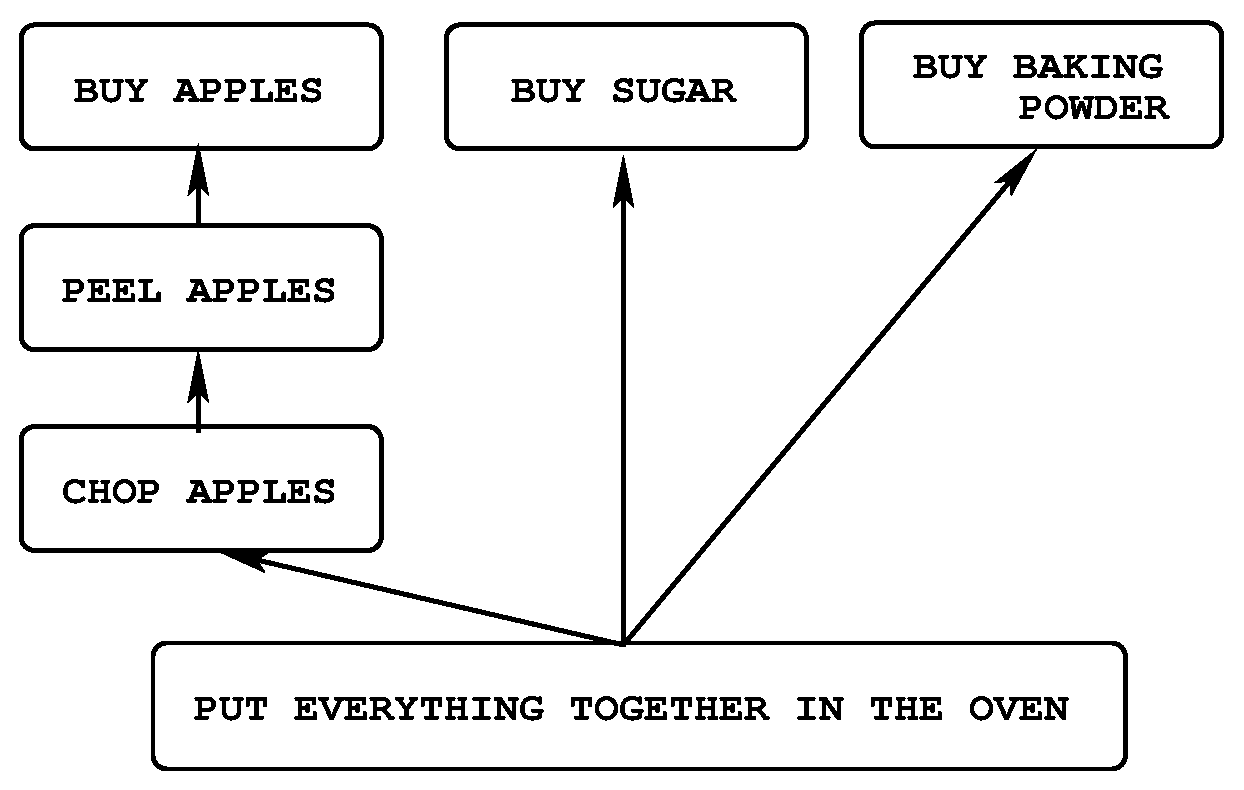
\includegraphics[height=0.45\paperheight]{figures/apple-pie}

\column[t]{0.38\textwidth}\pause
Possible translation:
\begin{itemize}
    \item Buy apples
    \item Buy suger
    \item Buy baking powder
    \item Peel apples
    \item Chop apples
    \item Put everything together in the oven
\end{itemize}
\end{columns}

%   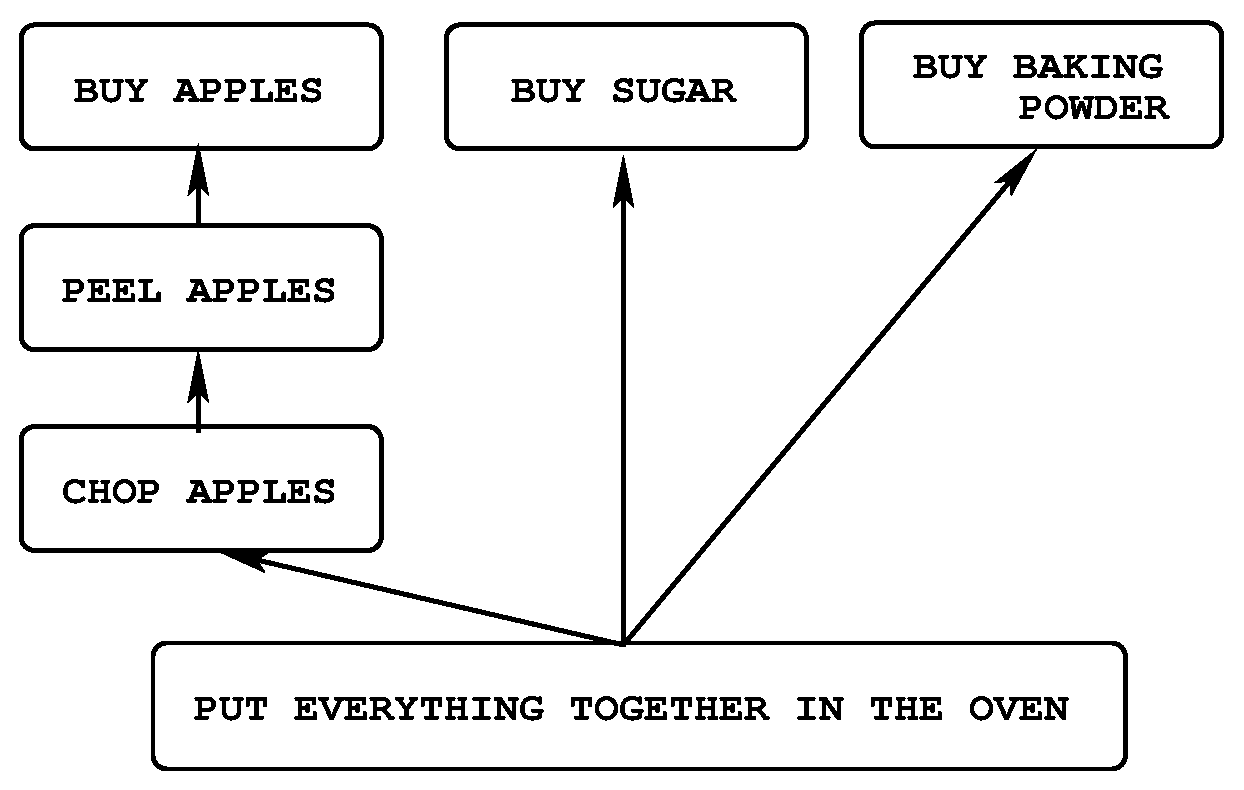
\includegraphics[height=0.45\paperheight]{figures/apple-pie}

\end{frame}


\begin{frame}[fragile,t]
  \frametitle{Structure}

\begin{itemize}
    \item Instruction-Level Parallelism: optimizing (single) pipeline execution:
            \begin{itemize}
                \item local code motion: within a basic block,
                \item cyclic code motion, e.g., loop unrolling.
               % \item non-cyclic code motion, e.g., predicated instructions.
               %%trace scheduling: schedule issued for the most likely 
               %%program trace based on static prediction (profiling) + compensation code 
               %%for all other possible traces.
            \end{itemize}
            \bigskip

    \item Reasoning about data-dependencies in loop nests:
            \begin{itemize}
                \item loop parallelism,
                \item loop interchange,
                \item loop distribution.
            \end{itemize}\bigskip

    \item Applications.
\end{itemize}

\end{frame}

\begin{frame}[fragile,t]
    \frametitle{Local Scheduling: Code Motion In a Basic Block}

Single-issue pipeline with separate integer and float execution:\bigskip

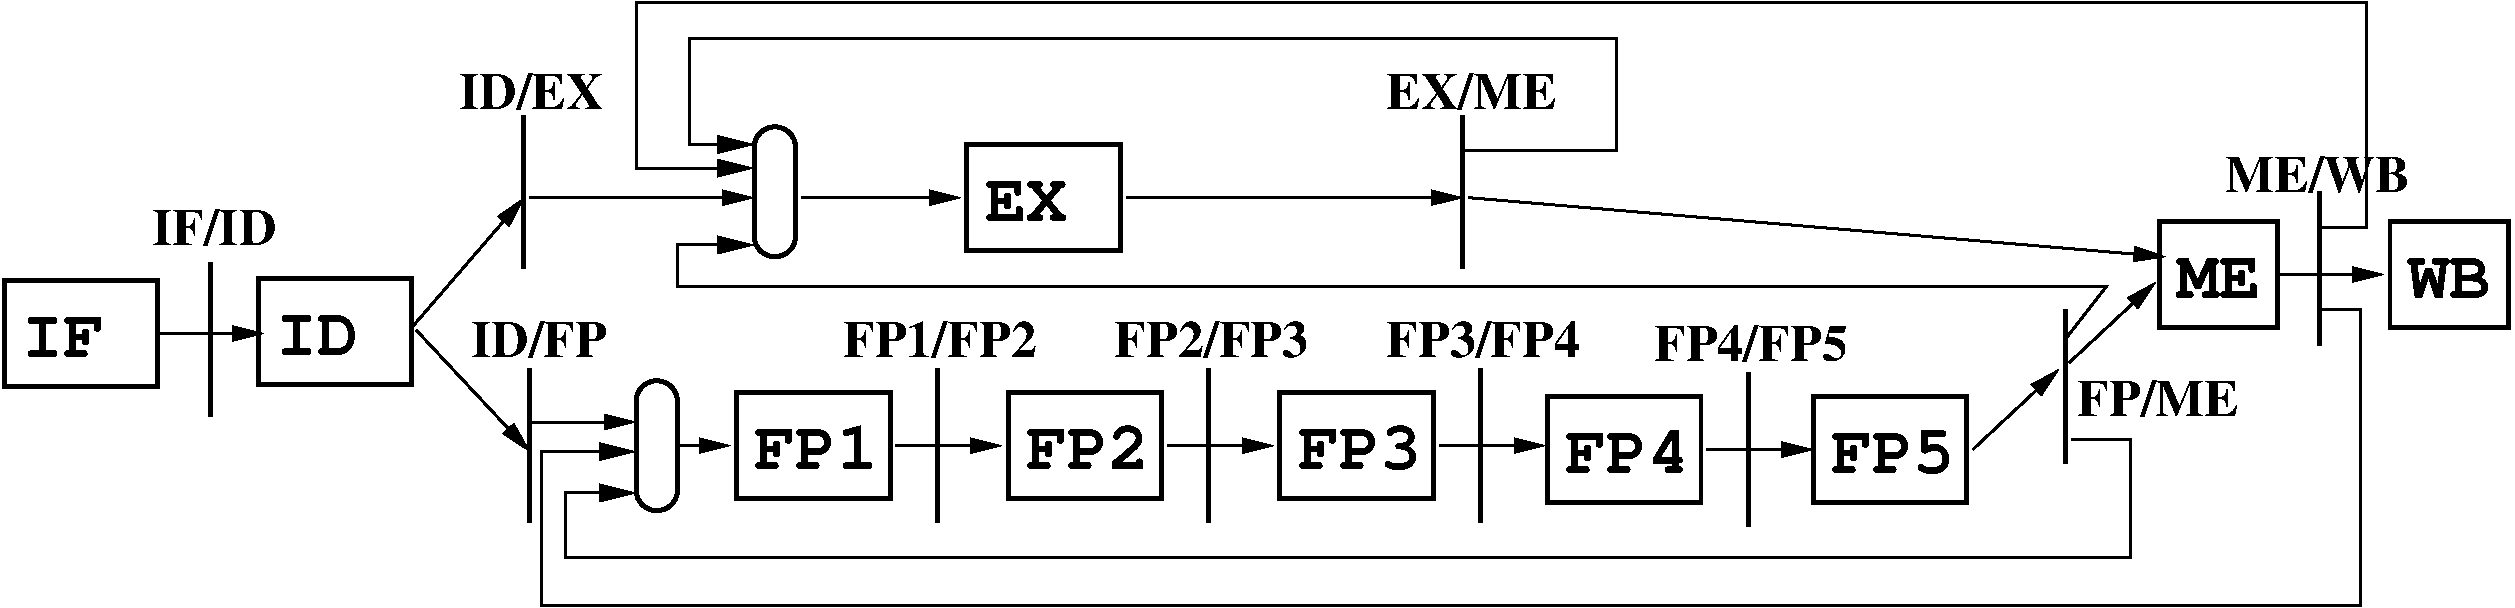
\includegraphics[width=53ex]{figures/SimpleOoOPipeline}
\bigskip


\begin{block}{HL Code{\tt~~~}Unoptimized}
\begin{columns}
\column{0.13\textwidth}
\begin{colorcode}[fontsize=\scriptsize]
for(i=0;
    i<100; 
    i++)
  A[i]=A[i]
      +B[i]
\end{colorcode} 
\column{0.38\textwidth}
\begin{colorcode}[fontsize=\scriptsize]
//R3=100, R1/2=@A/B 
L: L.S   F0, 0(R1)   (1)
   L.S   F1, 0(R2)   (1)
   \emp{ADD.S F2, F1, F0  (2)}
   \emp{S.S   F2, 0(R1)   (5)}
   ADDI  R1, R1, #4  (1)
   ADDI  R2, R2, #4  (1)
   SUBI  R3, R3, #1  (1)
   BNEZ  R3, L       (3)
\end{colorcode} 
\column{0.38\textwidth}
\begin{colorcode}[fontsize=\scriptsize]

\end{colorcode} 
\end{columns}
\end{block}
\end{frame}

\begin{frame}[fragile,t]
    \frametitle{Local Scheduling: Code Motion In a Basic Block}

\begin{block}{HL Code{\tt~~~}Unoptimized{\tt~~~~~~~~~}After Code Motion}
\begin{columns}
\column{0.13\textwidth}
\begin{colorcode}[fontsize=\scriptsize]
for(i=0;
    i<100;
    i++)
  A[i]=A[i]
      +B[i]
\end{colorcode} 
\column{0.38\textwidth}
\begin{colorcode}[fontsize=\scriptsize]
//R3=100, R1/2=@A/B 
L: L.S   F0, 0(R1)   (1)
   L.S   F1, 0(R2)   (1)
   \emp{ADD.S F2, F1, F0  (2)}
   \emp{S.S   F2, 0(R1)   (5)}
   ADDI  R1, R1, #4  (1)
   ADDI  R2, R2, #4  (1)
   SUBI  R3, R3, #1  (1)
   BNEZ  R3, Loop    (3)
\end{colorcode} 
\column{0.38\textwidth}
\begin{colorcode}[fontsize=\scriptsize]
//R3=100, R1/2=@A/B 
L: L.S   F0, 0(R1)   (1)
   L.S   F1, 0(R2)   (1)
   \emphh{SUBI  R3, R3, #1  (1)}    
   ADD.S F2, F1, F0  (1)
   ADDI  R1, R1, #4  (1)
   ADDI  R2, R2, #4  (1)
   \emphh{S.S   F2, -4(R1)  (3)}
   BNEZ  R3, Loop    (3)
\end{colorcode} 
\end{columns}
\end{block}

\emph{Unoptim\#clocks = 15, Optimized\#clocks = 12, Speedup = 1.25$\times$.}\medskip
\pause

\begin{itemize}
    \item {\tt SUB.I} \emp{moved up} after {\tt L.S} to eliminate the stall
            caused by a load followed by a dependent use. 
    \item {S.S} \emp{moved down} far away from the {ADD.S} it depends on, but
    \item introduces {\sc WAR} dependency, solved by adjusting {\tt S.S} 
            offset. 
\end  {itemize}

Move loads up, stores down and break apart dependent instructs.

\end{frame}

\begin{frame}[fragile,t]
    \frametitle{Cyclic Scheduling: Loop Unrolling}

Basic Blocks have on average 4-5 instructions $\Rightarrow$ limited benefits.
\smallskip

Loop Unrolling: schedules are computed across several iterations.

\begin{block}{Original{\tt~~~}Unroll Twice{\tt~~~}Rename Regs{\tt~~}Loads$\uparrow$ Stores$\downarrow$}
\begin{columns}
\column{0.15\textwidth}
\begin{colorcode}[fontsize=\scriptsize]
for(i=0;
i<100;i++)
  t1 = A[i]
  t2 = B[i]
  t3 = t1+t2
  A[i] = t3
\end{colorcode} 
\column{0.2\textwidth}
\begin{colorcode}[fontsize=\scriptsize]
for(i=0;
i<100;i+=2)
  t1 = A[i]
  t2 = B[i]
  t3 = t1+t2
  A[i] = t3
  \emp{t1 = A[i+1]}
  \emp{t2 = B[i+1]}
  \emp{t3 = t1+t2}
  \emp{A[i+1] = t3}
\end{colorcode} 
\column{0.22\textwidth}
\begin{colorcode}[fontsize=\scriptsize]
for(i=0;
i<100;i+=2)
  t1 = A[i]
  t2 = B[i]
  t3 = t1+t2
  \emp{A[i] = t3}
  \emphh{t4} = \emp{A[i+1]}
  \emphh{t5} = \emp{B[i+1]}
  \emphh{t6} = t4+t5
  A[i+1] = \emphh{t6}
\end{colorcode} 
\column{0.22\textwidth}
\begin{colorcode}[fontsize=\scriptsize]
for(i=0;
i<100;i+=2)
  t1 = \emphh{A[i]}
  t2 = \emphh{B[i]}
  t4 = \emphh{A[i+1]}
  t5 = \emphh{B[i+1]}
  t3 = t1+t2
  t6 = t4+t5
  \emphh{A[i]} = t3
  \emphh{A[i+1]} = t6
\end{colorcode} 
\end{columns}
\end{block}
\smallskip \pause

\begin{itemize}
    \item unroll twice, but epilog is required if unknown loop count,
    \item code motion in expanded body limited by WAW, WAR deps,
    \item which are fixed by {\bf \emph{renaming}} registers \& adjusting displs,
    \item finally, loads are moved up and stores down
\end{itemize}

\end{frame}

\begin{frame}[fragile,t]
    \frametitle{Loop Unrolling on a Single-Issue Pipeline}

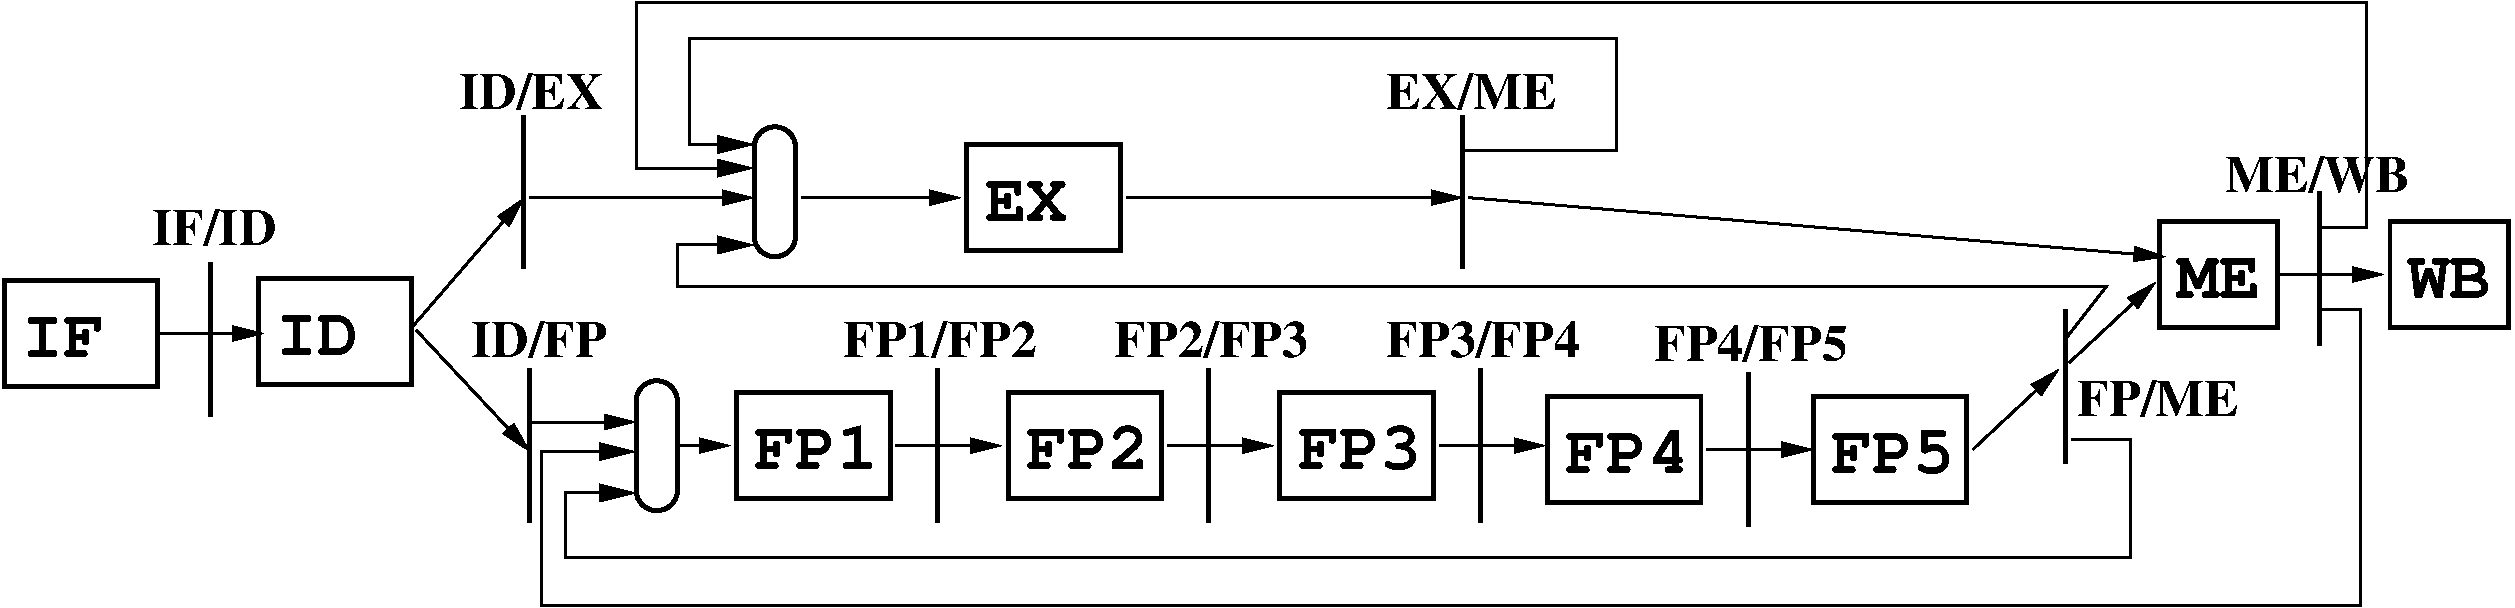
\includegraphics[width=50ex]{figures/SimpleOoOPipeline}

\begin{block}{TAC Optim Code{\tt~~~~~~~~}MIPS Optim Code}
\begin{columns}
\column{0.42\textwidth}
\begin{colorcode}[fontsize=\scriptsize]
for(i=0;i<100;i+=2)
  t1 = \emph{A[i]}
  t2 = \emph{B[i]}
  t4 = \emph{A[i+1]}
  t5 = \emph{B[i+1]}
  t3 = t1+t2
  t6 = t4+t5
  \emp{A[i]} = t3
  \emp{A[i+1]} = t6
\end{colorcode}
\column{0.55\textwidth}
\begin{colorcode}[fontsize=\scriptsize]
Loop: \emph{L.S   F0, 0(R1)}   (1)
      \emph{L.S   F1, 0(R2)}   (1) 
      \emph{L.S   F3, 4(R1)}   (1)
      \emph{L.S   F4, 4(R2)}   (1)
      ADD.S F2, F1, F0  (1)
      ADD.S F5, F3, F4  (1)
      SUBI  R3, R3, #2  (1)
      ADDI  R1, R1, #8  (1)
      ADDI  R2, R2, #8  (1)
      \emp{S.S   F2, -8(R1)}  (1)
      \emp{S.S   F5, -4(R1)}  (1)
      BNEZ  R3, Loop    (3)
\end{colorcode}  
\end{columns}
\end{block}
\smallskip 

% in paranthesis, number of clocks in ID
\# clocks for 2 iters: 14 $\Rightarrow$ Speedup = 15/7 = 2.14$\times$

\end{frame}

\begin{frame}[fragile,t]
  \frametitle{}

\huge{\center
Data-dependencies in loop nests:
            \begin{itemize}
                \item loop parallelism,
                \item loop interchange,
                \item loop distribution.
            \end{itemize}
}
\end{frame}

\begin{frame}[fragile,t]
  \frametitle{Data-Dependencies in Loop Nests} % of CPU, Multicores, GPGPU

%[fontsize=\small]
\begin{block}{Three Loop Examples}
\begin{colorcode}
DO i = 1, N         DO i = 2, N             DO i = 2, N
 DO j = 1, N         DO j = 2, N             DO j = 1, N 
  A[j,i] = A[j,i]..   A[j,i] = A[j-1,i-1]..   A[i,j] = A[i-1,j+1]..
 ENDDO                B[j,i] = B[j-1,i]..    ENDDO
ENDDO               ENDDO ENDDO             ENDDO
\end{colorcode}
\end{block} 

Iterations ordered {\em lexicographically}, i.e., in the order
they occur in the sequential execution, 
{\tt$\vec{k}=$(i=2,j=4) < $\vec{l}=$(i=3,j=3)}.

\bigskip

Would like to answer questions such as:
\begin{itemize}
    \item \emp{Which of the three loop nests is amenable to parallelization?}\smallskip
%    \item Loop interchange is one of the most simple and useful code transformations,
%            e.g., used to enhance locality of reference, parallel-loop granularity,
%            and even to ``create'' parallelism.\smallskip
    \item \emp{In which loop nest is it safe to interchange the loops?}
\end{itemize}


\end{frame}

\begin{frame}[fragile,t]
  \frametitle{Definition of a Dependency} % of CPU, Multicores, GPGPU

\begin{block}{Load-Store Classification of Dependencies}
\begin{colorcode}
True Dep. (RAW)      Anti Dep. (WAR)      Output dep. (WAW)
S1    X  = ..        S1    .. = X         S1    X = ...            
S2    .. = X         S2    X  = ..        S2    X = ...
\end{colorcode}
\end{block} 

\smallskip

{\bf Th. Loop Dependence:} There is a dependence from statement $S1$ to $S2$
in a loop nest {\em iff} $\exists$ iterations $\vec{k}$, $\vec{l}$ such that:\pause
\begin{description}
    \item[1.] $\vec{k} < \vec{l}$ or $\vec{k} = \vec{l}$ and $\exists$ 
                an execution path from statement $S1$ to statement $S2$ \emp{such that:}
    \item[2.] $S1$ accesses memory location $M$ on iteration $\vec{k}$, and
    \item[3.] $S2$ accesses memory location $M$ on iteration $\vec{l}$, and
    \item[4.] one of these accesses is a write.
\end{description}
\medskip

\emp{We say that $S1$ is the source and $S2$ is the sink of the dependence}. 
%because $S1$ executes before $S2$ in the sequential program execution.
Dependence depicted with an arrow pointing from source to sink.\pause

\bigskip
We are most interested in cross iteration dependencies, i.e., $\vec{k} < \vec{l}$.\\\smallskip
Intra iteration dependencies, i.e., $\vec{k} = \vec{l}$ are analysed for ILP. 

\end{frame}


\begin{frame}[fragile,t]
  \frametitle{Data-Dependencies in Loop Nests} % of CPU, Multicores, GPGPU

{\em Lexicographic ordering}, 
e.g., {\tt$\vec{k}=$(i=2,j=4) < $\vec{l}=$(i=3,j=3)}.

%[fontsize=\small]
\begin{block}{Three Loop Examples}
\begin{colorcode}
DO i = 1, N          DO i = 2, N              DO i = 2, N
 DO j = 1, N          DO j = 2, N              DO j = 1, N 
  A[j,i] = A[j,i]..    A[j,i] = A[j-1,i-1]..    A[i,j] = A[i-1,j+1]..
 ENDDO                 B[j,i] = B[j-1,i]..     ENDDO
ENDDO                ENDDO ENDDO              ENDDO
\end{colorcode}
\end{block} 
\pause

\hspace{-3ex}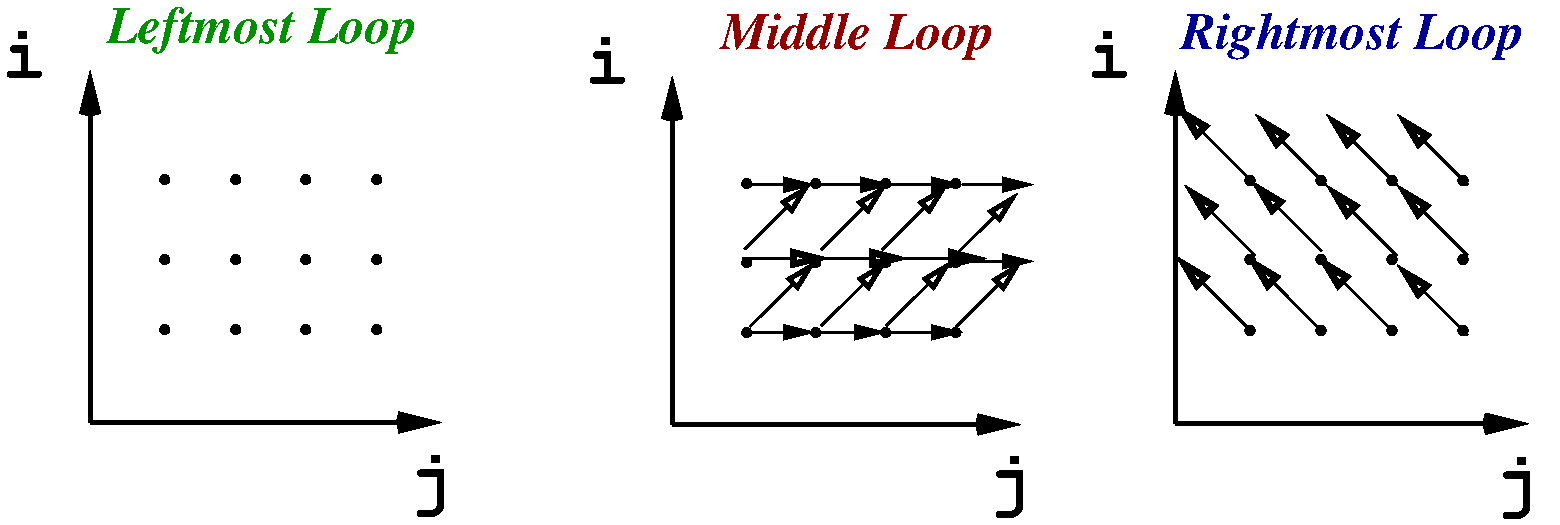
\includegraphics[height=20ex]{figures/LoopDeps}  

\alert{How can I summarize this information?} %Do I have to consider all cases?

\end{frame}





\begin{frame}[fragile,t]
  \frametitle{Summarize Dependence Info by Direction Vectors} % of CPU, Multicores, GPGPU

\begin{block}{Write the Direction Vectors for Each Loop:}
\begin{colorcode}
  DO i = 1, N            DO i = 2, N               DO i = 2, N
    DO j = 1, N            DO j = 2, N               DO j = 1, N 
S1    A[j,i]=A[j,i]..  S1   A[j,i]=A[j-1,i]...   S1    A[i,j]=A[i-1,j+1]...
    ENDDO              S2   B[j,i]=B[j-1,i-1]...     ENDDO
  ENDDO                  ENDDO ENDDO               ENDDO
\end{colorcode}
\end{block} 



\smallskip

%Dependencies depicted via an edge {\em from} the stmt that executes first
%in the loop nest, i.e., {\em the source}, {\em to} the one that executes later, {\em the sink}.

\smallskip

{\bf Def. Dependence Direction:} Assume $\exists$ a dependence from $S1$ in iteration $\vec{k}$
to $S2$ in $\vec{l}$ ($\vec{k}\leq\vec{l}$). 
\emp{\em Dependence-direction vector $\vec{D}(\vec{k},\vec{l})$}:
\begin{description}
    \item[1.] $\vec{D}(\vec{k},\vec{l})_m = $~``{\tt{}<}'' if $\vec{k}_m < \vec{l}_m$,
    \item[2.] $\vec{D}(\vec{k},\vec{l})_m = $~``{\tt{}=}'' if $\vec{k}_m = \vec{l}_m$,
    \item[3.] $\vec{D}(\vec{k},\vec{l})_m = $~``{\tt{}>}'' if $\vec{k}_m > \vec{l}_m$.
\end{description}

\medskip
If the source is a write and the sink a read then {\sc raw} dependency,\\If the source is a read then {\sc war}, if both are writes then {\sc waw}.  
\end{frame}


%\begin{frame}[fragile,t]
%  \frametitle{How to Compute the Direction Vectors?}
%\begin{itemize}
%    \item For any two statements $S1$ and $S2$ that may access the same
%            array $A$ (and one of the accesses is a write),\medskip
%    \item in two symbolic iterations $I^1\equiv(i^1_1,\ldots i^1_m)$
%            and $I^2=(i^2_1,\ldots i^2_m)$ (such that $I^1 < I^2$)\medskip
%    \item on indices $A[e^1_1,\ldots,e^1_n]$ and $A[e^2_1,\ldots,e^2_n]$,
%            respectivelly,\medskip
%    \item then \textbf{\it the direction vectors may be derived} from the equations\\
%            $\begin{cases}
%                e^1_1 = e^2_1\\
%                \ldots\\
%                e^1_n = e^2_n
%            \end{cases}$\\
%            (The system of equations models the definition of a dependency: 
%                both accesses need to refer to the same memory location!)
%\end{itemize}
%\end{frame}

\begin{frame}[fragile,t]
  \frametitle{Parallelism and Loop Interchange} % of CPU, Multicores, GPGPU

\begin{block}{Direction Vectors/Matrix for Three Loops }
\begin{columns}
\column{0.23\textwidth}
\begin{colorcode}
  DO i = 1, N
    DO j = 1, N
S1    A[j,i]=
       A[j,i]..
    ENDDO
  ENDDO
For S1\mymath{\rightarrow}S1: 
 (j1,i1)=(j2,i2) 
 i1\emp{=}i2 \& j1\emp{=}j2

Direction matrix:
S1\mymath{\rightarrow}S1: \emp{[=,=]}\pause
\end{colorcode}
\column{0.4\textwidth}
\begin{colorcode}
  DO i = 2, N
   DO j = 2, N
S1  A[j,i]=A[j-1,i]...
S2  B[j,i]=B[j-1,i-1]...
   ENDDO
  ENDDO
S1\mymath{\rightarrow}S1: (j1,i1)=(j2-1,i2)
        i1 \emp{=} i2 \& j1 \emp{<} j2
S2\mymath{\rightarrow}S2: (j1,i1)=(j2-1,i2-1)
        i1 \emp{<} i2 \& j1 \emp{<} j2
S1\mymath{\rightarrow}S1: \emp{[=,<]}
S2\mymath{\rightarrow}S2: \emp{[<,<]}\pause
\end{colorcode}
\column{0.23\textwidth}
\begin{colorcode}
  DO i = 2, N
   DO j = 1, N
S1  A[i,j]=
     A[i-1,j+1]...
   ENDDO
  ENDDO
For S1\mymath{\rightarrow}S1:
 (i1,j1)=(i2-1,
          j2+1)
 i1\emp{<}i2 \& j1\emp{>}j2

Direction matrix:
S1\mymath{\rightarrow}S1: \emp{[<,>]}\pause
\end{colorcode}
\end{columns}
\end{block} 

{\bf Th. Parallelism:} A loop in a loop nest is {\bf not} parallel {\em iff} the loop 
exhibits at least one non-{\tt{}=} direction such that all preceding directions 
(of outer loops) are {\tt =}.

\smallskip

\alert{A direction vector cannot have $>$ as the first non-= symbol},\\
as that would mean that I depend on something in the future. 
\end{frame}

\begin{frame}[fragile,t]
  \frametitle{Parallelism and Loop Interchange} % of CPU, Multicores, GPGPU

\begin{block}{Direction Vectors/Matrix for Three Loops }
\begin{columns}
\column{0.23\textwidth}
\begin{colorcode}
  DO i = 1, N
    DO j = 1, N
S1    A[j,i]=
       A[j,i]..
    ENDDO
  ENDDO
For S1\mymath{\rightarrow}S1: 
 (j1,i1)=(j2,i2) 
 i1\emp{=}i2 \& j1\emp{=}j2

Direction matrix:
S1\mymath{\rightarrow}S1: \emp{[=,=]}
\end{colorcode}
\column{0.4\textwidth}
\begin{colorcode}
  DO i = 2, N
   DO j = 2, N
S1  A[j,i]=A[j-1,i]...
S2  B[j,i]=B[j-1,i-1]...
   ENDDO
  ENDDO
S1\mymath{\rightarrow}S1: (j1,i1)=(j2-1,i2)
        i1 \emp{=} i2 \& j1 \emp{<} j2
S2\mymath{\rightarrow}S2: (j1,i1)=(j2-1,i2-1)
        i1 \emp{<} i2 \& j1 \emp{<} j2
S1\mymath{\rightarrow}S1: \emp{[=,<]}
S2\mymath{\rightarrow}S2: \emp{[<,<]}
\end{colorcode}
\column{0.23\textwidth}
\begin{colorcode}
  DO i = 2, N
   DO j = 1, N
S1  A[i,j]=
     A[i-1,j+1]...
   ENDDO
  ENDDO
For S1\mymath{\rightarrow}S1:
 (i1,j1)=(i2-1,
          j2+1)
 i1\emp{<}i2 \& j1\emp{>}j2

Direction matrix:
S1\mymath{\rightarrow}S1: \emp{[<,>]}
\end{colorcode}
\end{columns}
\end{block} 

{\bf Th. Loop Interchange:} A column-wise permutation of the loops in a loop nest 
is legal {\em iff} permuting the direction matrix in the same way {\em does NOT result}
in a {\tt >} direction as the leftmost non-{\tt{}=} direction in a row. 

\end{frame}


\begin{frame}[fragile,t]
  \frametitle{Parallelism and Loop Interchange} 

\begin{block}{Direction Vectors/Matrix for Three Loops }
\begin{columns}
\column{0.23\textwidth}
\begin{colorcode}
  DO i = 1, N
    DO j = 1, N
S1    A[j,i]=
       A[j,i]..
    ENDDO
  ENDDO
For S1\mymath{\rightarrow}S1: 
 (j1,i1)=(j2,i2) 
 i1\emp{=}i2 \& j1\emp{=}j2

Direction matrix:
S1\mymath{\rightarrow}S1: \emp{[=,=]}
\end{colorcode}
\column{0.4\textwidth}
\begin{colorcode}
  DO i = 2, N
   DO j = 2, N
S1  A[j,i]=A[j-1,i]...
S2  B[j,i]=B[j-1,i-1]...
   ENDDO
  ENDDO
S1\mymath{\rightarrow}S1: (j1,i1)=(j2-1,i2)
        i1 \emp{=} i2 \& j1 \emp{<} j2
S2\mymath{\rightarrow}S2: (j1,i1)=(j2-1,i2-1)
        i1 \emp{<} i2 \& j1 \emp{<} j2
S1\mymath{\rightarrow}S1: \emp{[=,<]}
S2\mymath{\rightarrow}S2: \emp{[<,<]}
\end{colorcode}
\column{0.23\textwidth}
\begin{colorcode}
  DO i = 2, N
   DO j = 1, N
S1  A[i,j]=
     A[i-1,j+1]...
   ENDDO
  ENDDO
For S1\mymath{\rightarrow}S1:
 (i1,j1)=(i2-1,
          j2+1)
 i1\emp{<}i2 \& j1\emp{>}j2

Direction matrix:
S1\mymath{\rightarrow}S1: \emp{[<,>]}
\end{colorcode}
\end{columns}
\end{block} 


Interchange is safe for first \& second nests, but not for the third!\\
e.g., \emp{\tt [=,<]}$~~~\Rightarrow~~~$ \emph{\tt [<,=]}$~~~~~~~~~$(for the second loop nest)\\
$~~~~~~~$\emp{\tt [<,<]}$~~~~~~~~~~~$\emph{\tt [<,<]}

\pause\smallskip

After interchange, loop $j$ of the second loop nest is parallel.

\bigskip

\emph{\bf Corollary: A parallel loop can be always interchanged inwards.}
\end{frame}


\begin{frame}[fragile,t]
  \frametitle{Dependency Graph and Loop Distribution} 

{\bf Def. Dependency Graph:} edges from the source of the dependency, i.e., early iteration, 
to the sink, i.e., later iteration. 

\smallskip

{\bf Th. Loop Distribution:} Statements that are in a dependence cycle remain in one 
(sequential) loop.   The others are distributed to separate loops in graph order; 
if no cycle then parallel loops.\smallskip

\begin{block}{Vectorization Example: Remember Vector Machines?}
\begin{columns}
\column{0.34\textwidth}
\begin{colorcode}[fontsize=\scriptsize]
  DO i = 3, N
\emp{S1  A[i] = B[i-2] ...}
\alert{S2  B[i] = B[i-1] ...}
  ENDDO  

For S2\mymath{\rightarrow}S1: i1 = i2-2, \emp{[<]}
For S2\mymath{\rightarrow}S2: i1 = i2-1, \emp{[<]}
\end{colorcode}
\column{0.27\textwidth}\pause
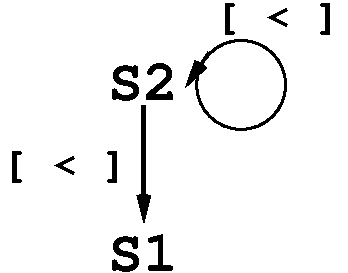
\includegraphics[height=12ex]{figures/LoopDistr}  
\column{0.30\textwidth}
\begin{colorcode}[fontsize=\scriptsize]
  \alert{DO} i = 3, N
S2  B[i] = B[i-1] ...
  \alert{ENDDO}

  \emphh{DOALL} i = 3, N
\emp{S1  A[i] = B[i-2] ...}
  \emphh{ENDDOALL}
\end{colorcode}
\end{columns}
\end{block}

\medskip

{\bf Corollary:} It is always legal to distribute a parallel loop;\\
\alert{but requires array expansion for local variables or if output
dependencies are present.}
\end{frame}

\begin{frame}[fragile,t]
  \frametitle{Applications of Data-Dependency Analysis}

\emphh{The discovered loop-level parallelism can be used for:}
\begin{itemize}
    \item parallel execution, e.g., multi/many cores (obvious)\medskip
    \item latency hiding, e.g., hardware multi-threading\medskip
    \item creating very-deep pipelines by vectorization + unrolling, 
            e.g., vector machines, FPGAs.\medskip
\end{itemize}\bigskip

\emphh{Loop interchange and distribution can be used for:}
\begin{itemize}
    \item locality-of-reference optimization, e.g., tiling
    \item enhancing the degree of flat parallelism
\end{itemize}

\end{frame}

\end{document}

%%% Local Variables:
%%% mode: latex
%%% TeX-master: t
%%% End:
